\section{Fundamentals of \gls{doris} System}\label{sec:doris-system-fundamentals}
In the late 1980s, \gls{cnes}, in conjunction with \gls{ign} and \gls{grgs} developed 
a new geodetic tracking system called \gls{doris} for precise orbit determination 
of \gls{leo} satellites for oceanographic missions. Since then, \gls{doris} has 
made huge leaps forward, and proved to be an invaluable tool to the scientific community, 
greatly expanding its application range and significance. This process lead in 
2003 to the creation of \gls{ids} (\cite{Willis2016a}), part of the \gls{ggos} 
within the \gls{iag} (\cite{Willis2006}). 

\begin{figure}
  \centering
  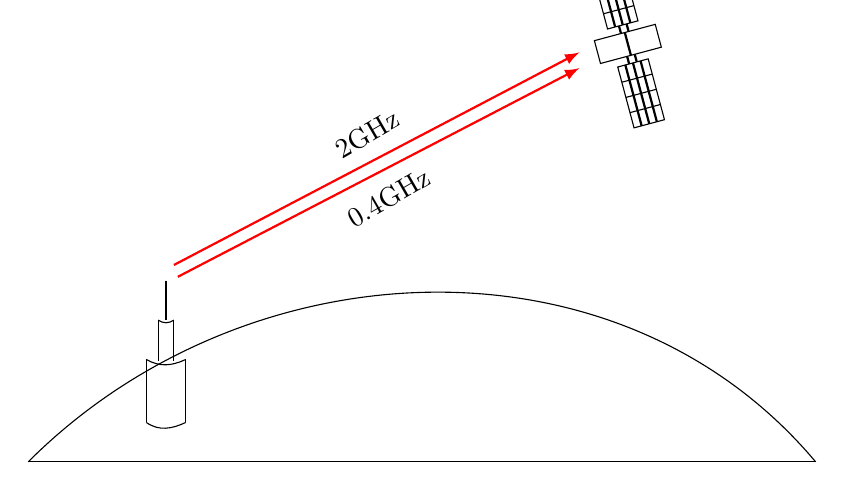
\begin{tikzpicture}
    \coordinate (lend) at (-5, 0);
    \coordinate (rend) at (5, 0);
    \draw (lend) to (rend);
    \draw (lend) to[out=45,in=-230] (rend);

    \coordinate (blb) at (-3.5, 0.5);
    \coordinate (brb) at (-3, 0.5);
    \draw (blb) to[out=-35,in=205] (brb);

    \coordinate (mlb) at (-3.5, 1.3);
    \coordinate (mrb) at (-3, 1.3);
    \draw (mlb) to[out=-30,in=205] (mrb);
    %\draw (mlb) to[out=35,in=-205] (mrb);
    \draw (blb) to (mlb);
    \draw (brb) to (mrb);
    
    \coordinate (tlb) at (-3.35, 1.8);
    \coordinate (trb) at (-3.15, 1.8);
    \draw (tlb) to[out=-35,in=215] (trb);
    \draw (tlb) to (-3.35, 1.28);
    \draw (trb) to (-3.15, 1.28);

    \coordinate (ulb) at (-3.26, 2.3);
    \coordinate (urb) at (-3.24, 2.3);
    \draw (ulb) to (-3.26, 1.8);
    \draw (urb) to (-3.24, 1.8);

    \rotatebox{15}{%
    \draw[] (3.5,4.6) rectangle (4.3,4.3);
    % Up panel
    \draw[thick] (3.9,4.3) to (3.9,4.6);
    \draw[thick] (3.85,4.6) to (3.85,4.7);
    \draw[thick] (3.95,4.6) to (3.95,4.7);
    \draw[] (3.7,5.5) rectangle (4.1,4.7);
    % grid
    \draw[thick] (3.8,4.7) to (3.8, 5.5); 
    \draw[thick] (3.9,4.7) to (3.9, 5.5); 
    \draw[thick] (4.0,4.7) to (4.0, 5.5); 
    \draw[] (3.7,4.9) to (4.1, 4.9);
    \draw[] (3.7,5.1) to (4.1, 5.1);
    \draw[] (3.7,5.3) to (4.1, 5.3);
    % Down panel
    \draw[thick] (3.85,4.3) to (3.85,4.2);
    \draw[thick] (3.95,4.3) to (3.95,4.2);
    \draw[] (3.7,3.4) rectangle (4.1,4.2);
    % grid
    \draw[thick] (3.8,3.4) to (3.8, 4.2); 
    \draw[thick] (3.9,3.4) to (3.9, 4.2); 
    \draw[thick] (4.0,3.4) to (4.0, 4.2); 
    \draw[] (3.7,3.6) to (4.1, 3.6);
    \draw[] (3.7,3.8) to (4.1, 3.8);
    \draw[] (3.7,4.0) to (4.1, 4.0);
    }
    
    \coordinate (satant1) at (2.0,  5.2);
    \coordinate (bcnant1) at (-3.15,2.5);
    \coordinate (satant2) at (2.0,  5.0);
    \coordinate (bcnant2) at (-3.10,2.35);
    \draw[thick,red,-latex] (bcnant1) -- node[above=1mm, align=center, black, rotate=30]{2GHz} (satant1);
    \draw[thick,red,-latex] (bcnant2) -- node[below=1mm, align=center, black, rotate=30]{0.4GHz} (satant2);

\end{tikzpicture}

  \caption{\gls{doris} System Description}
  \label{fig:doris-system-description}
\end{figure}

\gls{doris} (\cite{Barlier2005}) originated during the design phase of the US-French 
TOPEX/Poseidon mission (\cite{Fu1994}), 
and constitutes a Doppler up-link system, optimized for orbit determination (both 
in real-time and post-processed). Radio signals are generated from a ground-tracking 
network, and Doppler measurements are performed on-board the satellite. Since its 
initialization, the system's technology has greatly improved, and its applications 
have gradually and logically expanded from orbit determination to gravity-field 
determination, terrestrial reference frame maintenance and geodynamics. Since TOPEX/Poseidon, an 
ever-increasing number of \gls{leo} satellite missions are equipped with on-board 
\gls{doris} receivers. \autoref{fig:doris-constellations} depicts past, current and 
future \gls{doris}-equipped satellite missions.

\begin{figure}[h!]
  \centering
  \includegraphics[height=.4\textheight,keepaspectratio]{Constellation2021}
  \caption{DORIS-ecquiped satellites; image courtesy of \gls{ids}.}
  \label{fig:doris-constellations}
\end{figure}

\gls{doris} is based on the accurate measurement of the Doppler shift of radio 
frequency signals transmitted from ground beacons and received on board the 
satellite(s) (\autoref{fig:doris-system-description}). Roughly every \SI{10}{\second}, 
the on-board receiver accurately measures 
the Doppler shift of radio-frequencies signals continuously transmitted from 
beacons at two frequencies: at \SI{2.03625}{\GHz} for precise Doppler measurement 
and at \SI{401.25}{\MHz} for correction of the propagation delay trough the 
ionosphere. The two channels are also used for time-tagging measurements and 
auxiliary data transmission (\cite{Auriol2010}).

\iffalse
\begin{description}
  \item[Atmospheric Studies] including troposphere () and ionosphere ()
  \item[Reference Frames] \cite{Willis2007}
  \item[Space Weather and Solar Activity] \cite{Willis2005}
  \item[Tectonics] \cite{}
\end{description}
\fi

\subsection{The \gls{doris} Tracking Network}\label{ssec:doris-tracking-network}
The tracking network is a key factor in the success of the \gls{doris} system. 
This network was established and is actively maintained by \gls{ign} and it currently 
(Feb. 2023) consists of $\approx 60$ sites (\autoref{fig:doris-network}). It is global, dense 
and homogeneous, and thus unique among the different techniques that contribute to 
\gls{itrf}. Since its establishment, very few changes of sites and/or instrumentation 
have been performed, thus enforcing network stability. Furthermore, it is (spatially) 
dense and well distributed geographically (especially between the Northern and  
Southern hemispheres). This spatial balance along with several collocations with 
other space-geodetic techniques (\autoref{fig:doris-network-ties}), make the 
\gls{doris} system an integral part of reference frame maintenance (\cite{Moreaux2022}).

\begin{figure}[h]
  \centering
  \includegraphics[height=.4\textheight,keepaspectratio]{permanent_network_Nov2020}
  \caption{The \gls{doris} Network (as of Nov. 2020); image courtesy of \gls{ids}.}
  \label{fig:doris-network}
\end{figure}

The strengths and advantages of the \gls{doris} tracking network, can be summarized 
by (\cite{Soudarin2019})
\begin{description}
  \item[Centralized control and management] of the network deployment and evolution, 
    including site instrumentation.
  \item[Long operation time]; time-series of current stations span a 21 year period in average, 
    with a median of 26.4 years.
  \item[Homogeneous spatial distribution]; half of the stations are located on 
    islands or coastal areas and the network is well balanced between the 
    Northern and Southern hemispheres (\autoref{fig:doris-network}).
  \item[Large number of co-locations]; 48 stations are co-located with 
    other techniques (\gls{gnss}: 47, \gls{slr}: 10, \gls{vlbi}: 7), plus 28 are 
    co-located with tide gauges (\autoref{fig:doris-network-ties})
\end{description}

\begin{figure}[h]
  \centering
  \includegraphics[height=.4\textheight,keepaspectratio]{colocation_IERS_TG_Nov2020}
  \caption{\gls{doris} stations co-located with other space-geodetic techniques 
    and tide-gauges (as of Nov. 2020); image courtesy of \gls{ids}.}
  \label{fig:doris-network-ties}
\end{figure}

\subsection{The \gls{ids}}\label{ssec:ids}
\gls{ids} was established in 2003, with the mission to (\cite{Soudarin2019})
\begin{itemize}
  \item provide support to research activities in geodesy and geophysics, based 
    on \gls{doris} data and derived products, and
  \item give access to data, products and documents related to the \gls{doris} system
\end{itemize}

The service is based on international cooperation on a volunteer basis and just like 
its geodetic counterparts (i.e. \gls{igs}, \gls{ilrs} and \gls{ivs} for \gls{gnss}, 
\gls{slr} and \gls{vlbi} respectively) plays a crucial role in the development of 
the technique and most importantly drives and facilitates its usage from the scientific 
community. Major products published by \gls{ids} include times series of the \gls{doris} 
tracking stations, along with their positions and velocities  and time series of 
geocenter motion and Earth orientation parameters. \gls{ids} also coordinates the 
technique's contribution to the \gls{itrf} (see e.g. \cite{Moreaux2022}).

\gls{ids}'s organization chart, includes a Governing Board and a Central Bureau.
The Analysis Centers process the \gls{doris} data available at the \gls{ids} Data 
Centers and generate products with the assistance of the Analysis Center Coordinator.
The \gls{ids} Combination Center provides regular combination of products of 
the Analysis Centers and is also in charge of the realization of the so-called 
DPOD (\gls{doris} extension to the current \gls{itrf} for \gls{pod}) 
which contains update mean positions and velocities of all the \gls{doris} stations. 
Last but not least, the \gls{ids} Combination Center produces the technique's 
contribution the \gls{itrf}.

\iffalse
\fi
